\resizebox{\columnwidth}{!}{
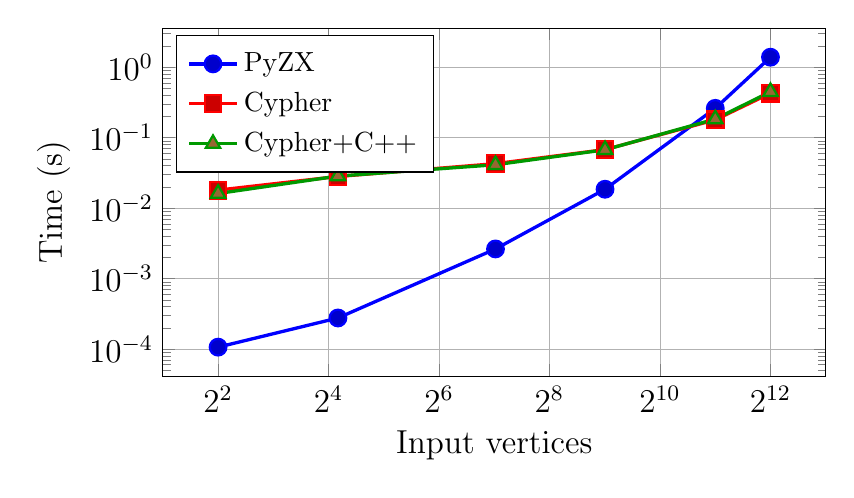
\begin{tikzpicture}
  \begin{axis}[
    width=10cm, height=6cm,
    xlabel={Input vertices}, ylabel={Time (s)},
    xmode=log, ymode=log, log basis x=2,
    grid=major,
    grid style={line width=.1pt, draw=gray!30},
    major grid style={line width=.2pt, draw=gray!60},
    label style={font=\large}, tick label style={font=\large},
    legend style={at={(0.02,0.98)}, anchor=north west,
      font=\normalsize, inner sep=4pt, row sep=2pt, cells={anchor=west}},
    legend image post style={mark size=3pt},
    every axis plot/.append style={line width=1.2pt, mark size=3pt,
      mark options={line width=0.8pt}},
    unbounded coords=jump,
  ]
    \addplot+[mark=*, color=blue, solid,error bars/.cd,y dir=both,y explicit] coordinates {
      (4,0.0001065)
      (18,0.0002762)
      (130,0.0026379)
      (514,0.0185804)
      (2050,0.2614747)
      (4098,1.3897561)
    };
    \addlegendentry{PyZX}

    \addplot+[mark=square*, color=red, solid,error bars/.cd,y dir=both,y explicit] coordinates {
      (4,0.0180403)
      (18,0.0281712)
      (130,0.0428462)
      (514,0.067814)
      (2050,0.1795511)
      (4098,0.4287933)
    };
    \addlegendentry{Cypher}

    \addplot+[mark=triangle*, color=green!60!black, solid,error bars/.cd,y dir=both,y explicit] coordinates {
      (4,0.0161625)
      (18,0.0285431)
      (130,0.0413427)
      (514,0.067426)
      (2050,0.1840216)
      (4098,0.4495195)
    };
    \addlegendentry{Cypher+C++}

  \end{axis}
\end{tikzpicture}
}
